\section*{Introduction}
Exploratory behavior can have two very different explanations depending on the expected result. If reward is expected, then exploration is explained as a search for reward \cite{Gupta2006,Sutton2018,Woodgate2017,Lee2011a,Schulz2018a,Calhoun2014}. This is how exploration is commonly framed \cite{Sutton2018}. 

If there is no reason to expect a reward, exploration is considered as a search for information, as curiosity \cite{Berlyne1950,Schmidhuber1991,Kidd2015,Jaegle2019,Sumner2019,Wang2019,Auersperg2015}. For example, when a rat is placed in a new maze it will explore, extensively, even if no food or water is expected \cite{Rosenberg2021}.

An open problem in the decision sciences is to unify exploration, of any kind, with exploitation (a.k.a, choosing most rewarding action). When exploration optimizes for reward value or reward information, as is common, this union leads to the famous exploration-exploitation dilemma \cite{Kelly1956,Berger-Tal2014,Dayan1996,Thrun1992,Mehlhorn2015,Kobayashi2019} which we illustrate in Fig. \ref{fig:bee}a. In this paper, we offer an alternative approach by unifying reward exploitation with curiosity. We illustrate this alternative in Fig. \ref{fig:bee}b.  

It is easy to justify our use of curiosity, in this way. Curiosity is a primary drive in most animals \cite{Berlyne1950,Loewenstein1994,Inglis2001}. It is a drive that is as strong as the drive for reward, if not stronger \cite{Loewenstein1994,Kidd2015,Gottlieb2018,Sumner2019,Gopnik2020,Song2019,Wang2019}. 

The first half of this paper we develop the theory behind our union. This consists of mathematical study of curiosity alone, and our mathematical solution to unifying curiosity with reward collection. The second half consists of initial simulations where we demonstrate performance which is as good, if not better, than more standard approaches. We conclude with some questions and answers about our approach.

\begin{figure}
	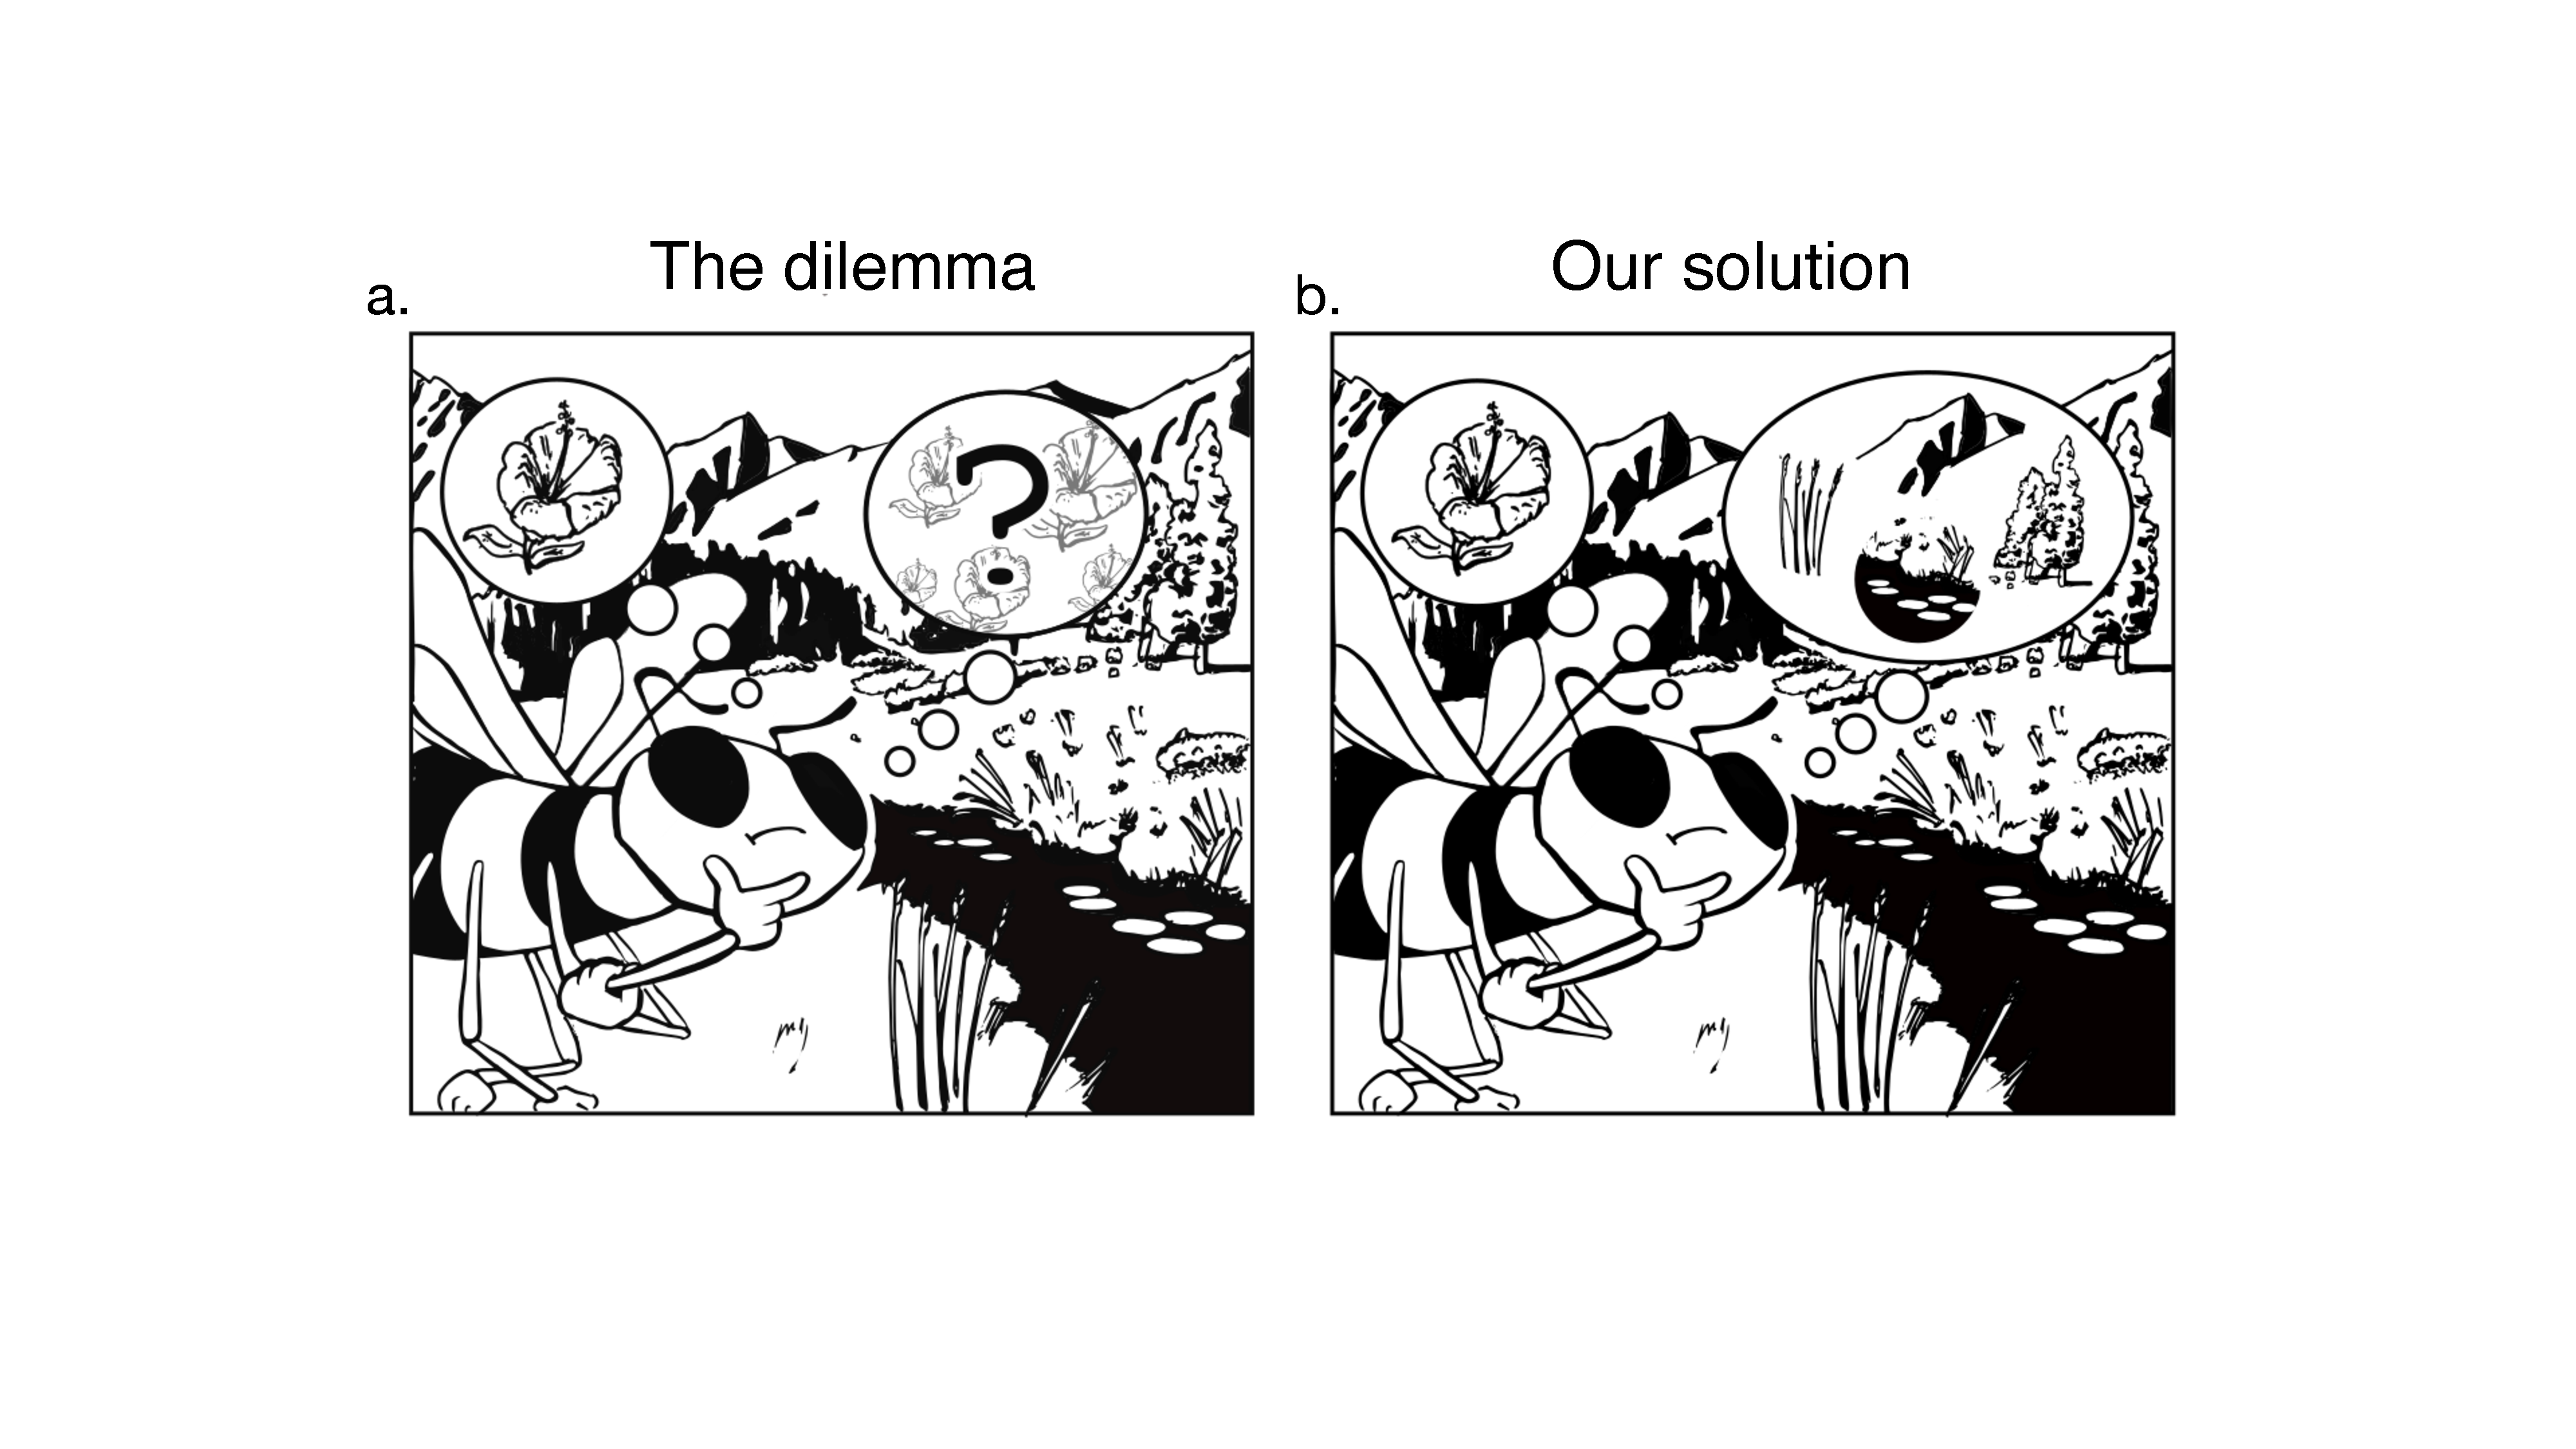
\includegraphics[width=.9\linewidth]{img/bee.pdf} 
	\caption{Two views of exploration and exploitation. \textbf{a}. The dilemma: either exploit an action with a known reward (e.g., return to the previous flower) or explore other actions on the chance they will return a better outcome. The central challenge here is that the outcome of exploration is uncertain, and filled with questions. \textbf{b}. An alternative view of the dilemma, with two goals: either maximize rewards \textit{or} maximize information value, with a curious search of the environment. \textit{Artist credit}: Richard Grant.}
	\label{fig:bee} 
\end{figure}

